\documentclass[12pt,mathserif,aspectratio=169]{beamer}
\usepackage[brazil]{babel}
\usepackage[utf8]{inputenc}
\usepackage[T1]{fontenc}
\usepackage{lmodern}
\usepackage{latexsym}
\usepackage{amssymb}
\usepackage{amsmath}
\usepackage{mathtools}
\usepackage{graphicx}
\usepackage{url}
\usepackage[portuguese,onelanguage,ruled]{algorithm2e}
\usepackage{hyperref}
\usepackage{ulem}

%%% CODE %%%
\usepackage{listings}
\usepackage{color}

\definecolor{codegreen}{rgb}{0,0.6,0}
\definecolor{codegray}{rgb}{0.5,0.5,0.5}
\definecolor{codepurple}{rgb}{0.58,0,0.82}
\definecolor{backcolour}{rgb}{0.95,0.95,0.92}

\lstdefinestyle{mystyle}{
	backgroundcolor=\color{backcolour},
	commentstyle=\color{codegreen},
	keywordstyle=\color{magenta},
	numberstyle=\tiny\color{codegray},
	stringstyle=\color{codepurple},
	basicstyle=\footnotesize,
	breakatwhitespace=false,
	breaklines=true,
	captionpos=b,
	keepspaces=true,
	numbers=left,
	numbersep=5pt,
	showspaces=false,
	showstringspaces=false,
	showtabs=false,
	tabsize=2
}

\lstset{style=mystyle}
%%% CODE %%%

\usecolortheme{whale}
\useoutertheme{infolines}
\setbeamertemplate{headline}[default]
\setbeamertemplate{caption}{\insertcaption}
\setbeamertemplate{navigation symbols}{}
\centering

\title[Introdução ao Aprendizado de Máquina]{Introdução ao Aprendizado de Máquina}
\author[Prof. Erneson A. Oliveira]{Prof. Erneson A. Oliveira$^*$}
\institute[MBACD-UNIFOR]{MBA em Ciência de Dados\\Universidade de Fortaleza}
\date{26 de Março de 2021}

\begin{document}

%%% TITLE %%%
\begin{frame}
    \vspace{1.0cm}
    \titlepage
    \vspace{-1.5cm}
    
    \begin{figure}
        \begin{minipage}{0.4\paperwidth}
            \vspace{1.75cm}
            \begin{flushleft}
                {\tiny $^*$ erneson@unifor.br}
            \end{flushleft}
        \end{minipage}
        \hfill
        \begin{minipage}{0.4\paperwidth}
            \vspace{-0.5cm}
            \begin{flushright}
                \includegraphics[width=0.2\paperwidth]{fig/UNIFOR.jpg}
            \end{flushright}
        \end{minipage}
    \end{figure}
\end{frame}
%%% TITLE %%%

%%% SLIDE %%%
\begin{frame}
	\Large Aula 1 - Introdução ao Aprendizado de Máquina (II)
	\begin{figure}
		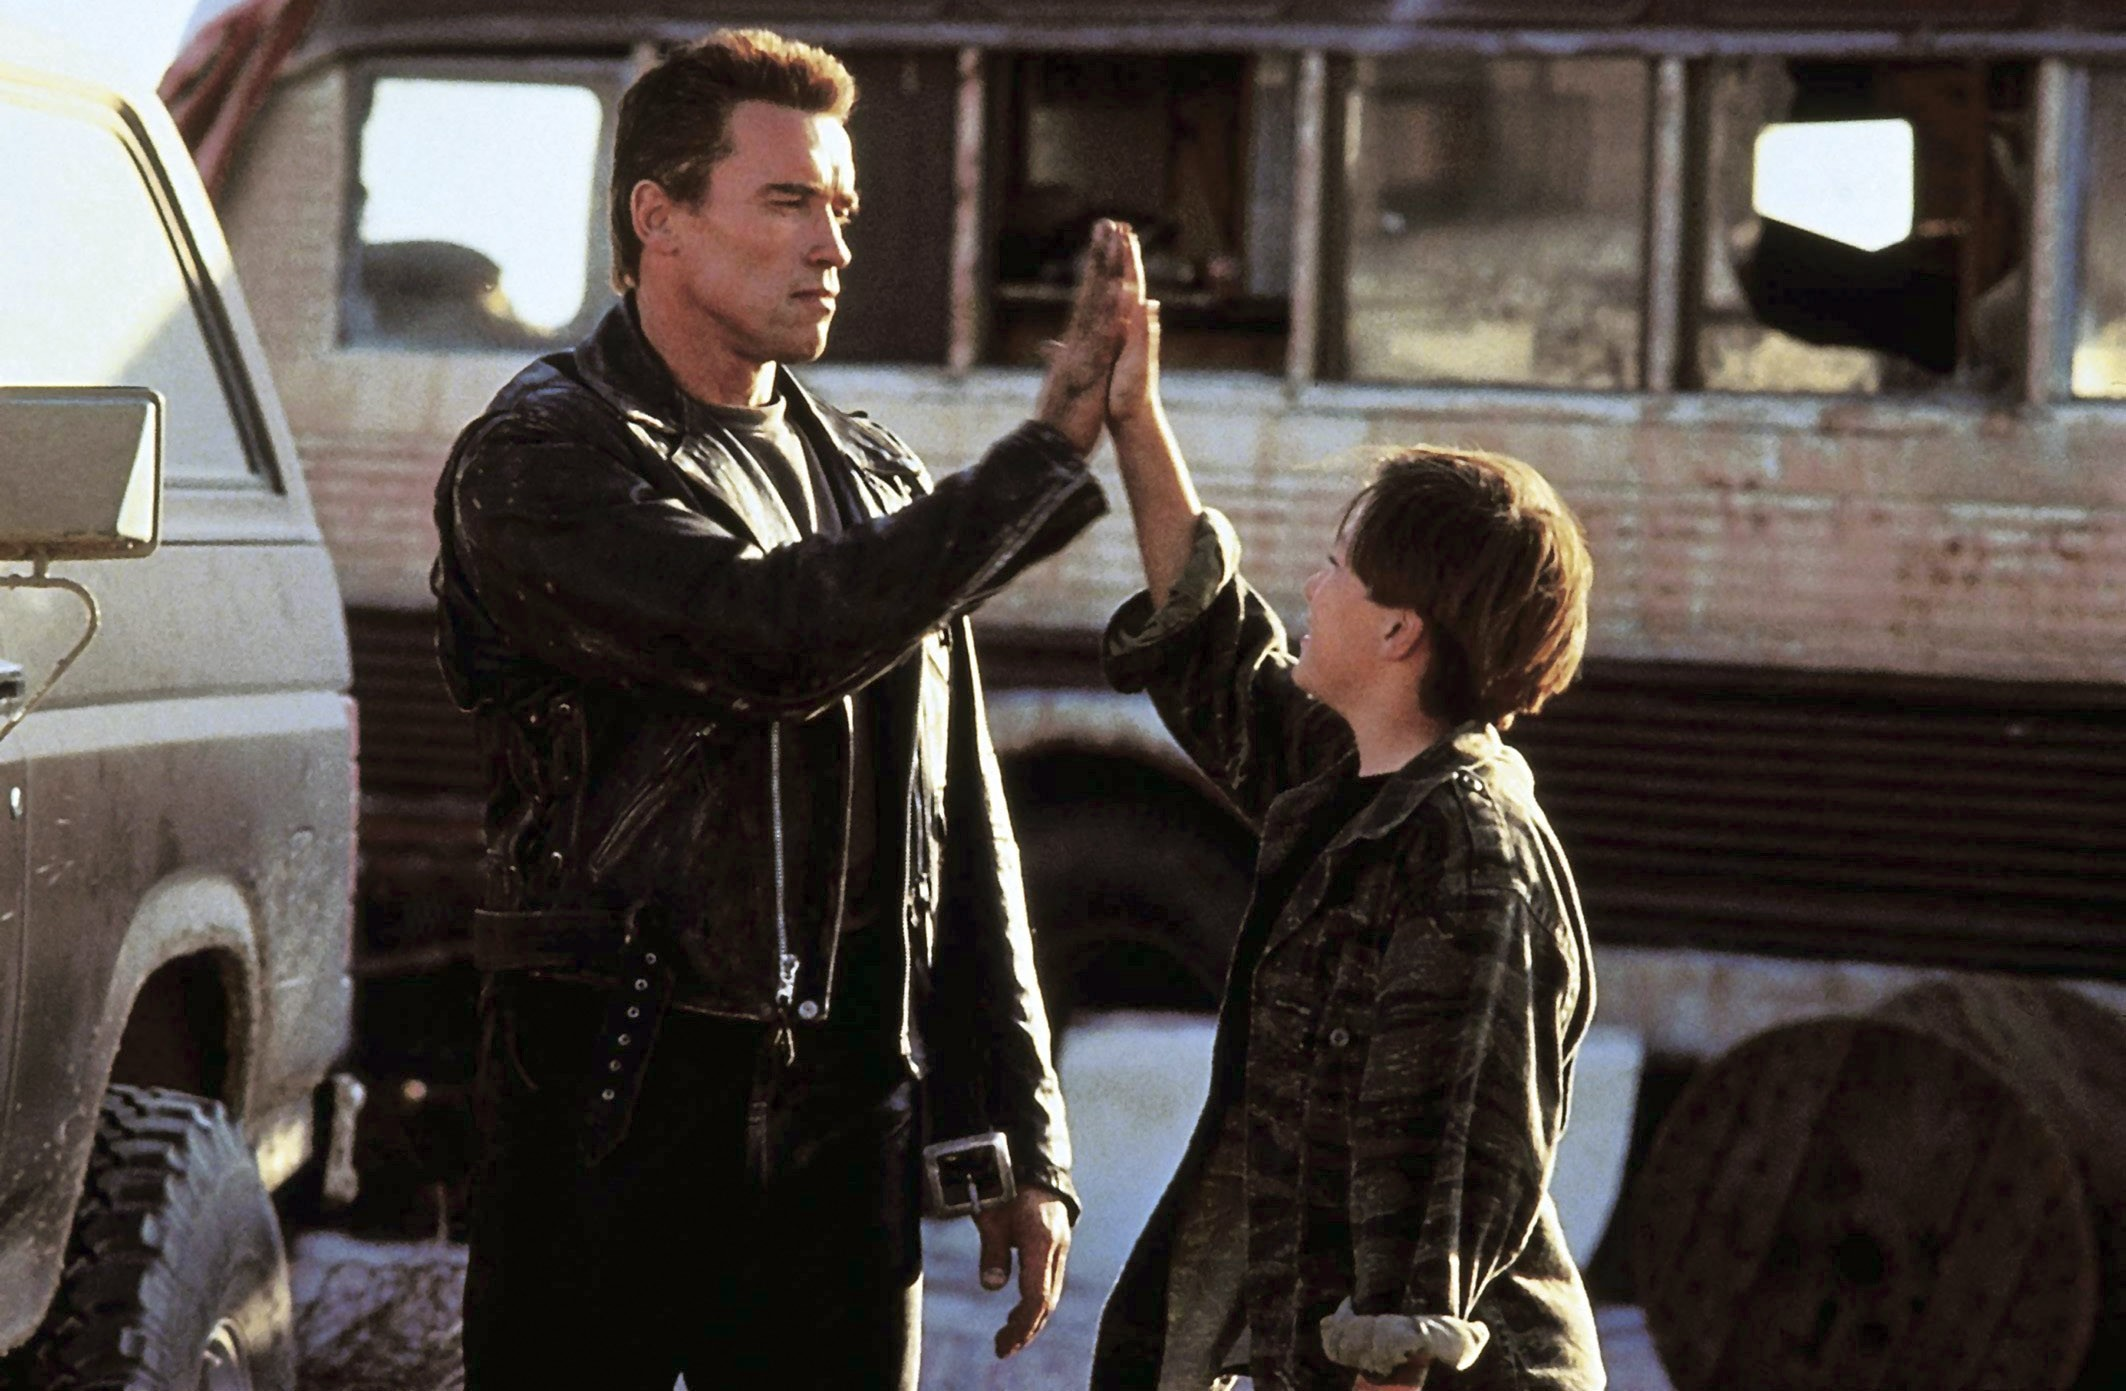
\includegraphics[width=0.7\paperwidth]{fig/terminator2.jpg}
	\end{figure}
\end{frame}
%%% SLIDE %%%

%%% SLIDE %%%
\begin{frame}
	\Huge Tipos de sistemas de AM (SAM)
\end{frame}
%%% SLIDE %%%

%%% SLIDE %%%
\begin{frame}{Tipos de Sistemas de AM (SAM)}
    \only<1-3>{
	    \begin{itemize}
            \uncover<1->{\item SAM treinados ou não com supervisão humana: Aprendizado supervisionado, aprendizado não-supervisionado, aprendizado semi-supervisionado e aprendizado por reforço;}
	        \uncover<2->{\item SAM que aprendem ou não em tempo real: Aprendizado em lote ({\it offline}) e aprendizado {\it online};}
	        \uncover<3->{\item SAM que funcionam comparando novos dados a dados conhecidos ou detectando padrões no conjunto de treinamento e construindo um modelo preditivo: Aprendizado baseado em instância e aprendizado baseado em modelo.}
	    \end{itemize}
    }
\end{frame}
%%% SLIDE %%%

%%% SLIDE %%%
\begin{frame}
	\Huge SAM treinados ou não com supervisão humana
\end{frame}
%%% SLIDE %%%

%%% SLIDE %%%
\begin{frame}
	\Huge Aprendizado supervisionado
\end{frame}
%%% SLIDE %%%

%%% SLIDE %%%
\begin{frame}{Aprendizado supervisionado}
    \only<1>{
        \begin{itemize}
            \item Conjunto de treinamento rotulado!
		\end{itemize}
		
		\begin{figure}
			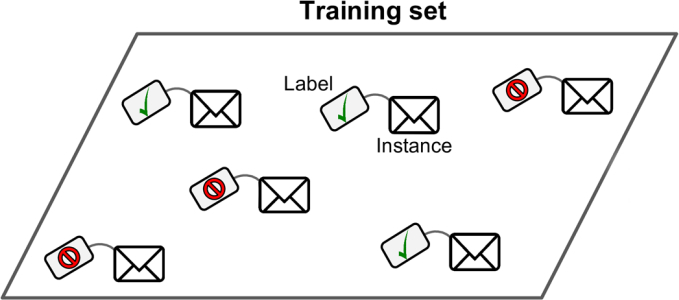
\includegraphics[width=0.6\textwidth]{fig/fig1_05a.jpg}
		\end{figure}
		
		\begin{itemize}
            \item O SAM é treinado para aprender com a supervisão humana.
	    \end{itemize}
	}
	
    \only<2>{
		\Large Classificação
    }
    
    \only<3>{
        \begin{itemize}
            \item Conjunto de treinamento: Rótulos e instâncias.
		\end{itemize}
		
		\begin{figure}
			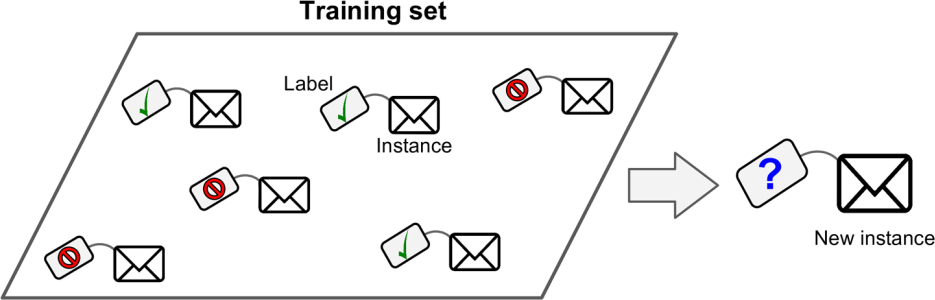
\includegraphics[width=0.6\textwidth]{fig/fig1_05.jpg}
		\end{figure}
		
		\begin{itemize}
            \item O SAM é treinado para classificar novas instâncias como pertencentes a uma determinada classe.
	    \end{itemize}
	}
	
	\only<4>{
		\Large Regressão
    }
	
	\only<5>{
	    \begin{itemize}
            \item Conjunto de treinamento: rótulos e características (ou atributos).
		\end{itemize}
		
		\begin{table}%[tbhp]
            \centering
            \begin{tabular}{c|c|c|c|c|c}
            {\bf Modelo}  & {\bf Quilometragem (km)} & {\bf Ano}    & {\bf Marca}      & \dots  & {\bf Valor (R\$)}\\
            \hline
            Corolla       & $1\;000$                 & 2019         & Toyota           & \dots  & $60\;000$\\
            Fusca         & $100\;000$               & 1984         & Volkswagem       & \dots  & $2\;000$\\
            Onix          & $15\;000$                & 2017         & Chevrolet        & \dots  & $30\;000$\\
            \vdots        & \vdots                   & \vdots       & \vdots           & \vdots & \vdots\\
            Duster        & $10\;000$                & 2018         & Renault          & \dots  & $45\;000$
            \end{tabular}
        \end{table}
	}
	
	\only<6>{
        \begin{figure}
			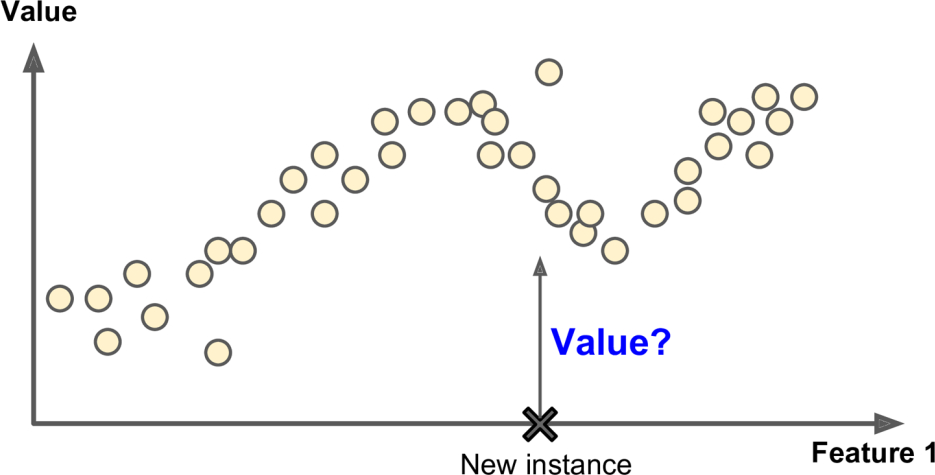
\includegraphics[width=0.6\textwidth]{fig/fig1_06.jpg}
		\end{figure}
		
        \begin{itemize}
	        \item O SAM é treinado para prever um valor numérico alvo (rótulo) de uma nova instância dado um conjunto de características.
	    \end{itemize}
    }
    
    \only<7>{
        Alguns dos mais importantes algoritmos de aprendizado supervisionado:
        
        \begin{itemize}
            \item k-Vizinhos Mais Próximos;
            \item Regressão Linear;
            \item Regressão Logística;
            \item Máquinas de Vetor de Suporte;
            \item Árvores de Decisão e Florestas Aleatórias;
            \item Redes Neurais.
	    \end{itemize}
    }
\end{frame}
%%% SLIDE %%%

%%% SLIDE %%%
\begin{frame}
	\Huge Aprendizado não-supervisionado
\end{frame}
%%% SLIDE %%%

%%% SLIDE %%%
\begin{frame}{Aprendizado não-supervisionado}
    \only<1>{
        \begin{itemize}
            \item Conjunto de treinamento não-rotulado!
		\end{itemize}
		
		\begin{figure}
			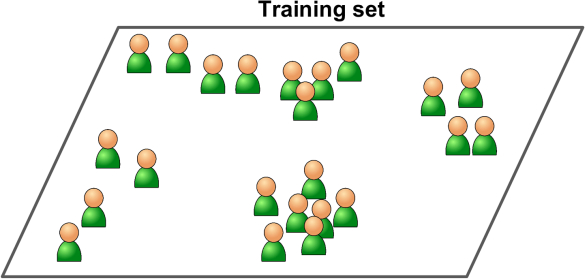
\includegraphics[width=0.6\textwidth]{fig/fig1_07.jpg}
		\end{figure}
		
		\begin{itemize}
            \item O SAM é treinado para aprender sem a supervisão humana.
	    \end{itemize}
	}
	
    \only<2>{
		\Large Agrupamento
    }
    
    \only<3>{
		\begin{figure}
			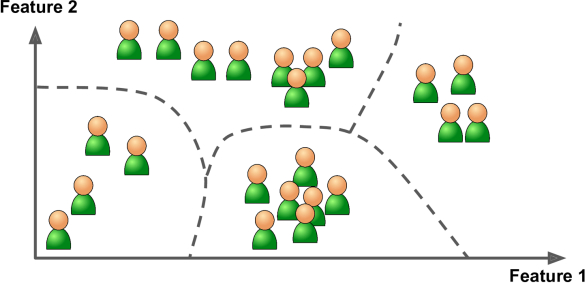
\includegraphics[width=0.6\textwidth]{fig/fig1_08.jpg}
		\end{figure}
		
		\begin{itemize}
            \item O SAM é treinado para detectar grupos de elementos parecidos ({\it e.g.} Seguidores no Twitter).
	    \end{itemize}
	}
	
	\only<4>{
		\Large Visualização
    }
	
	\only<5>{
		\begin{figure}
			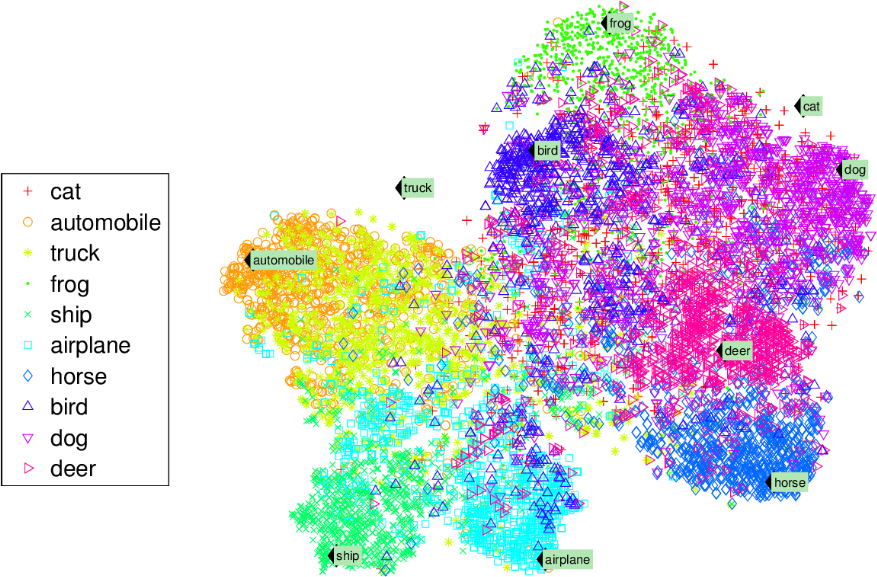
\includegraphics[width=0.5\textwidth]{fig/fig1_09.jpg}
		\end{figure}
		
		\begin{itemize}
            \item O SAM é treinado para representar o seu dado graficamente de forma mais intuitiva ({\it e.g.} Aglomerados semânticos).
	    \end{itemize}
	}
	
	\only<6>{
		\Large Redução de Dimensionalidade
    }
	
	\only<7>{
		\begin{table}%[tbhp]
            \centering
            \begin{tabular}{c|c|c|c|c|c}
            {\bf Modelo}  & {\bf Quilometragem (km)} & \sout{{\bf Ano}}    & {\bf Marca}      & \dots  & {\bf Valor (R\$)}\\
            \hline
            Corolla       & $1\;000$                 & \sout{2019}         & Toyota           & \dots  & $60\;000$\\
            Fusca         & $100\;000$               & \sout{1984}         & Volkswagem       & \dots  & $2\;000$\\
            Onix          & $15\;000$                & \sout{2017}         & Chevrolet        & \dots  & $30\;000$\\
            \vdots        & \vdots                   & \vdots              & \vdots           & \vdots & \vdots\\
            Duster        & $10\;000$                & \sout{2018}         & Renault          & \dots  & $45\;000$
            \end{tabular}
        \end{table}
		
		\begin{itemize}
            \item O SAM é treinado para simplificar o dado sem perder tanta informação (Extração de característica).
	    \end{itemize}
	}
	
	\only<8>{
		\Large Detecção de Anomalia (ou {\it Outliers})
    }
	
	\only<9>{
		\begin{figure}
			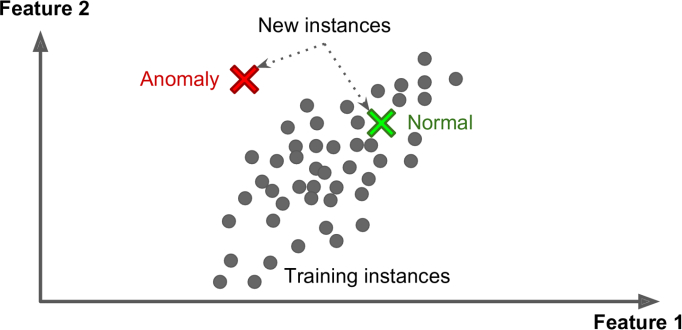
\includegraphics[width=0.6\textwidth]{fig/fig1_10.jpg}
		\end{figure}
		
		\begin{itemize}
            \item O SAM é treinado para identificar comportamentos anormais ({\it e.g.} Operações bancárias suspeitas).
	    \end{itemize}
	}
	
	\only<10>{
		\Large Regra de Associação
    }
    
    \only<11>{
		\begin{figure}
			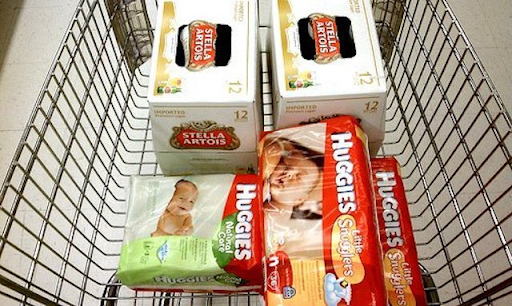
\includegraphics[width=0.6\textwidth]{fig/market_basket.jpg}
		\end{figure}
		
		\begin{itemize}
            \item O SAM é treinado para identificar relações de interesse ({\it e.g.} Cestas de compras).
	    \end{itemize}
	}
    
    \only<12>{
        Alguns dos mais importantes algoritmos de aprendizado não-supervisionado:
        
        \begin{itemize}
            \item {\it k-Means};
            \item Análise de agrupamento hierárquico;
            \item Maximização da expectativa;
            \item Análise de Componentes Principais;
            \item {\it Locally-linear embedding} (LLE);
            \item {\it t-distributed Stochastic Neighbor Embedding} (t-SNE);
            \item Apriori;
            \item Eclat.
	    \end{itemize}
    }
\end{frame}
%%% SLIDE %%%

%%% SLIDE %%%
\begin{frame}
	\Huge Aprendizado semi-supervisionado
\end{frame}
%%% SLIDE %%%

%%% SLIDE %%%
\begin{frame}{Aprendizado semi-supervisionado}
    \begin{itemize}
        \item Conjunto de treinamento parcialmente rotulado!
	\end{itemize}
	
	\begin{figure}
		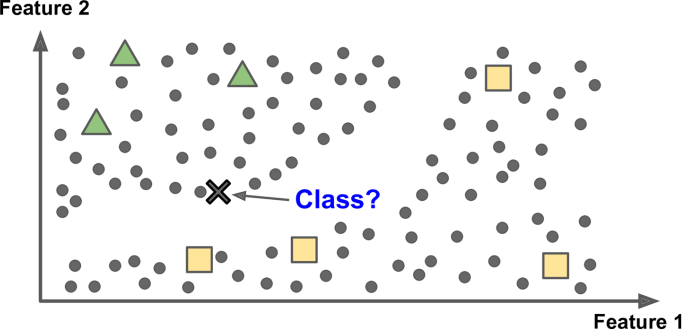
\includegraphics[width=0.6\textwidth]{fig/fig1_11.jpg}
	\end{figure}
	
	\begin{itemize}
        \item O SAM é treinado para aprender através de uma combinação de aprendizado supervisionado e não-supervisionado ({\it e.g.} Fotos no Facebook).
    \end{itemize}
\end{frame}
%%% SLIDE %%%

%%% SLIDE %%%
\begin{frame}
	\Huge Aprendizado por reforço
\end{frame}
%%% SLIDE %%%

%%% SLIDE %%%
\begin{frame}{Aprendizado por reforço}
    \only<1-3>{
	    \begin{minipage}{0.40\paperwidth}
	        \begin{itemize}
                \uncover<1->{\item Ambiente (conjunto de treinamento) e Agente (SAM);}
                \uncover<2->{\item O agente pode observar o ambiente, selecionar e realizar ações ganhando recompensas (ou sofrendo penalidades);}
                \uncover<3->{\item O agente é treinado para aprender a melhor estratégia (política).}
		    \end{itemize}
        \end{minipage}
        \begin{minipage}{0.50\paperwidth}
            \begin{figure}
			    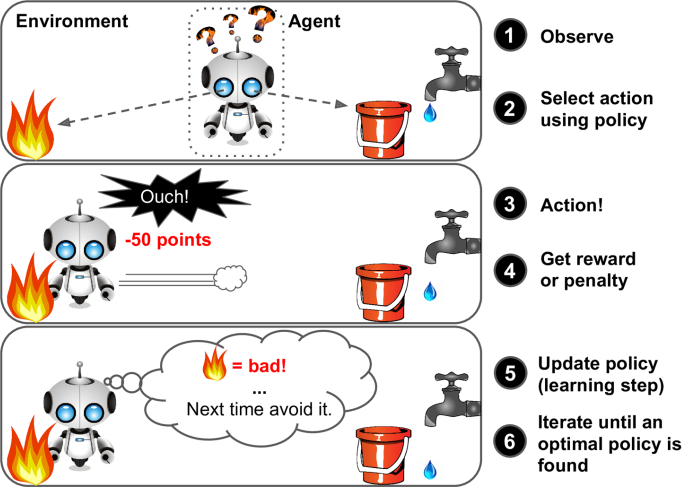
\includegraphics[width=1.0\textwidth]{fig/fig1_12.jpg}
		    \end{figure}
        \end{minipage}
	}
    
    \only<4>{
        \begin{figure}
			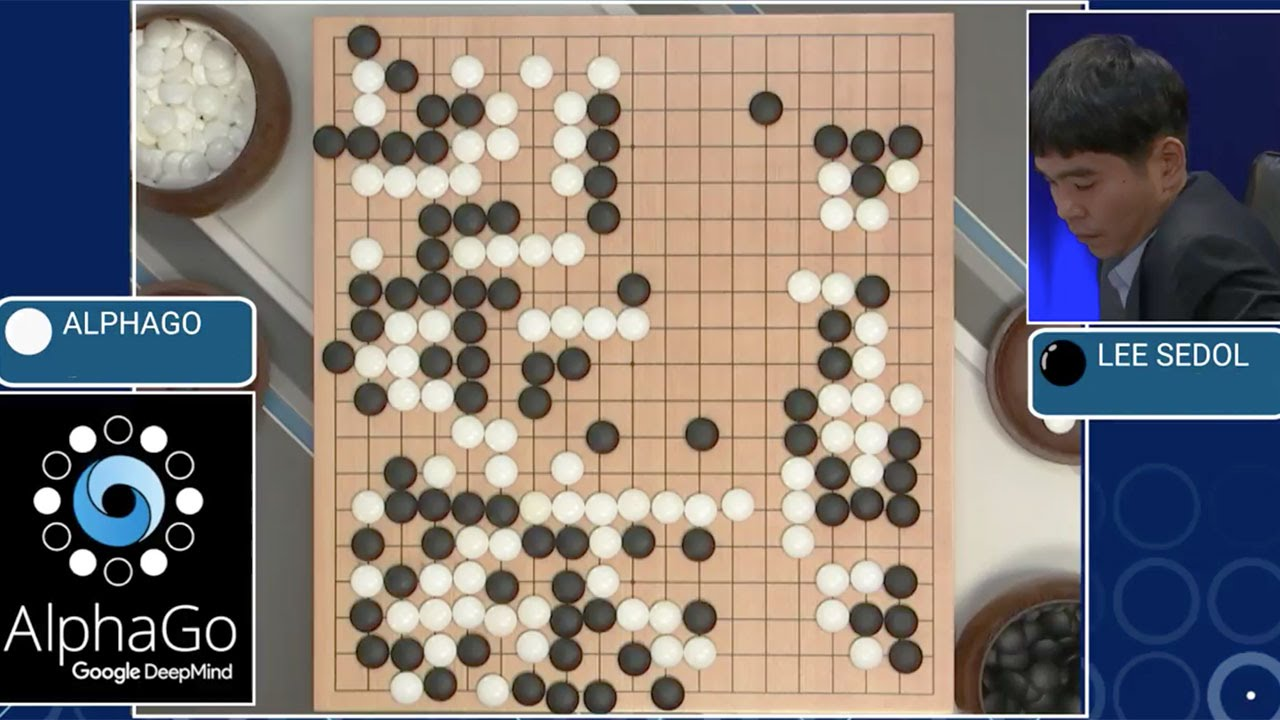
\includegraphics[width=0.8\textwidth]{fig/alphago.jpg}
		\end{figure}
    }
\end{frame}
%%% SLIDE %%%

%%% SLIDE %%%
\begin{frame}
	\Huge SAM que aprendem ou não em tempo real
\end{frame}
%%% SLIDE %%%

%%% SLIDE %%%
\begin{frame}
	\Huge Aprendizado em Lote ({\it offline})
\end{frame}
%%% SLIDE %%%

%%% SLIDE %%%
\begin{frame}{Aprendizado em Lote (offline)}
    \begin{figure}
		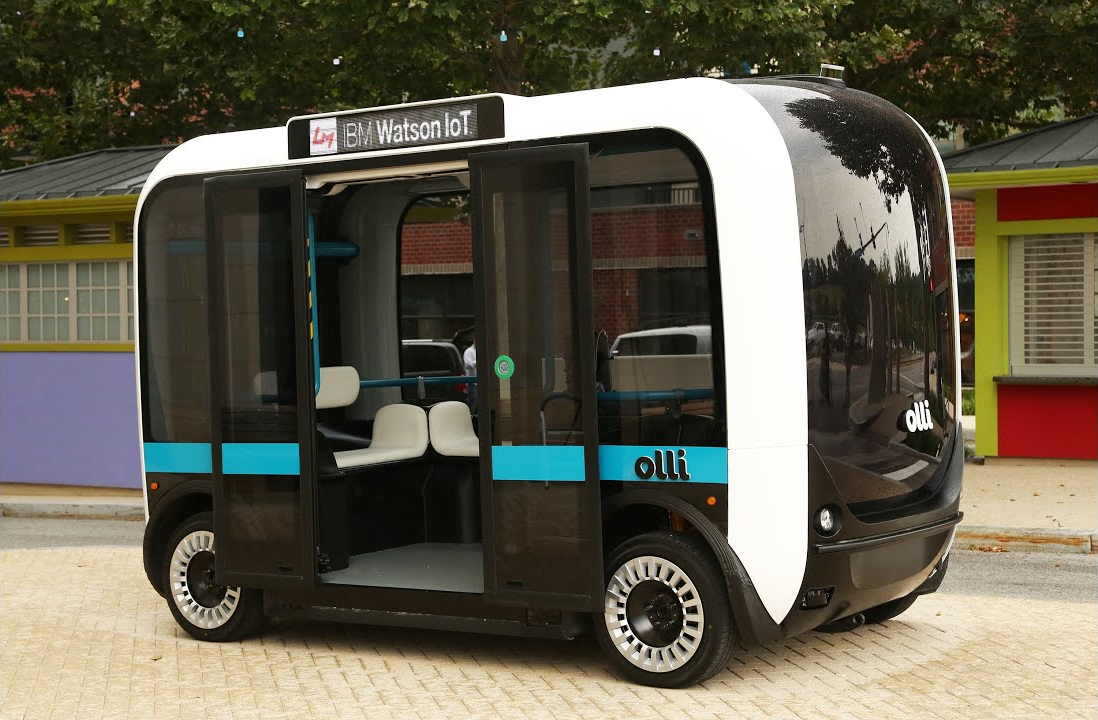
\includegraphics[width=0.6\textwidth]{fig/olli.jpg}
	\end{figure}
	
	\begin{itemize}
        \item O SAM é treinado com todos os dados disponíveis e lançado em produção.
    \end{itemize}
\end{frame}
%%% SLIDE %%%

%%% SLIDE %%%
\begin{frame}
	\Huge Aprendizado {\it online}
\end{frame}
%%% SLIDE %%%

%%% SLIDE %%%
\begin{frame}{Aprendizado online}
    \only<1>{
        \begin{figure}
			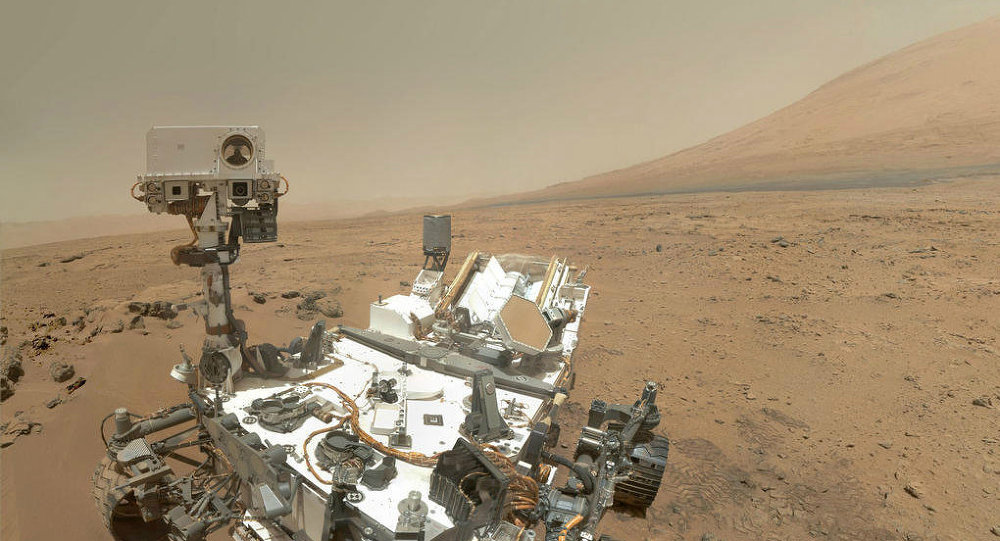
\includegraphics[width=0.7\textwidth]{fig/curiosity.jpg}
		\end{figure}
		
		\begin{itemize}
            \item O SAM é lançado em produção e treinado continuamente por novos dados.
	    \end{itemize}
    }
    
    \only<2>{
        \begin{figure}
			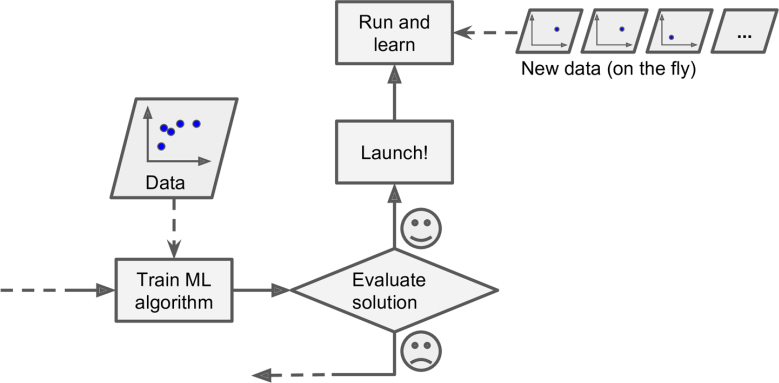
\includegraphics[width=0.7\textwidth]{fig/fig1_13.jpg}
		\end{figure}
		
		\begin{itemize}
            \item Taxa de Aprendizado: O quão veloz o SAM se adapta à mudanças nos dados.
	    \end{itemize}
    }
\end{frame}
%%% SLIDE %%%

%%% SLIDE %%%
\begin{frame}
	\Huge SAM que usam comparações de dados ou modelo preditivo
\end{frame}
%%% SLIDE %%%

%%% SLIDE %%%
\begin{frame}
	\Huge Aprendizado baseado em instância
\end{frame}
%%% SLIDE %%%

%%% SLIDE %%%
\begin{frame}{Aprendizado baseado em instância}
    \only<1>{
        \begin{figure}
			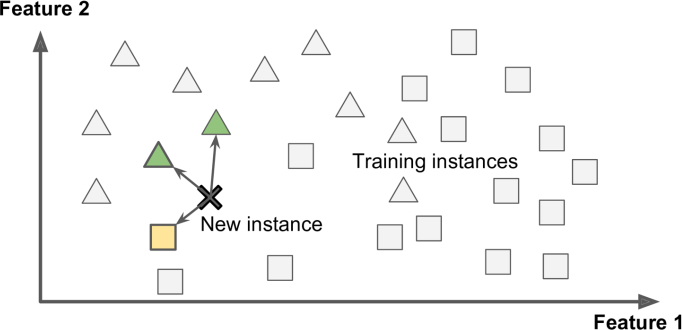
\includegraphics[width=0.8\textwidth]{fig/fig1_15.jpg}
		\end{figure}
		
		\begin{itemize}
            \item Medida de Similaridade: O quão similar, dado um critério, são duas instâncias.
	    \end{itemize}
    }
\end{frame}
%%% SLIDE %%%

%%% SLIDE %%%
\begin{frame}
	\Huge Aprendizado baseado em modelo
\end{frame}
%%% SLIDE %%%

%%% SLIDE %%%
\begin{frame}{Aprendizado baseado em modelo}
    \begin{figure}
		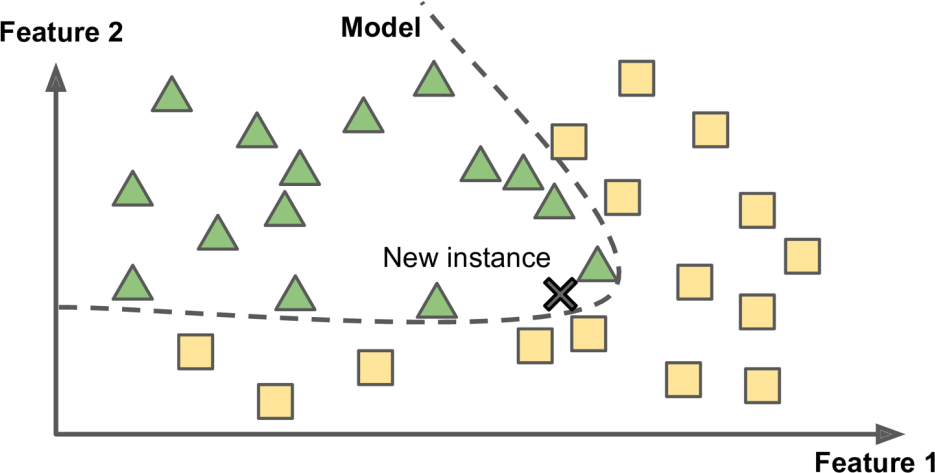
\includegraphics[width=0.8\textwidth]{fig/fig1_16.jpg}
	\end{figure}
\end{frame}
%%% SLIDE %%%

%%% SLIDE %%%
\begin{frame}
    \begin{figure}
        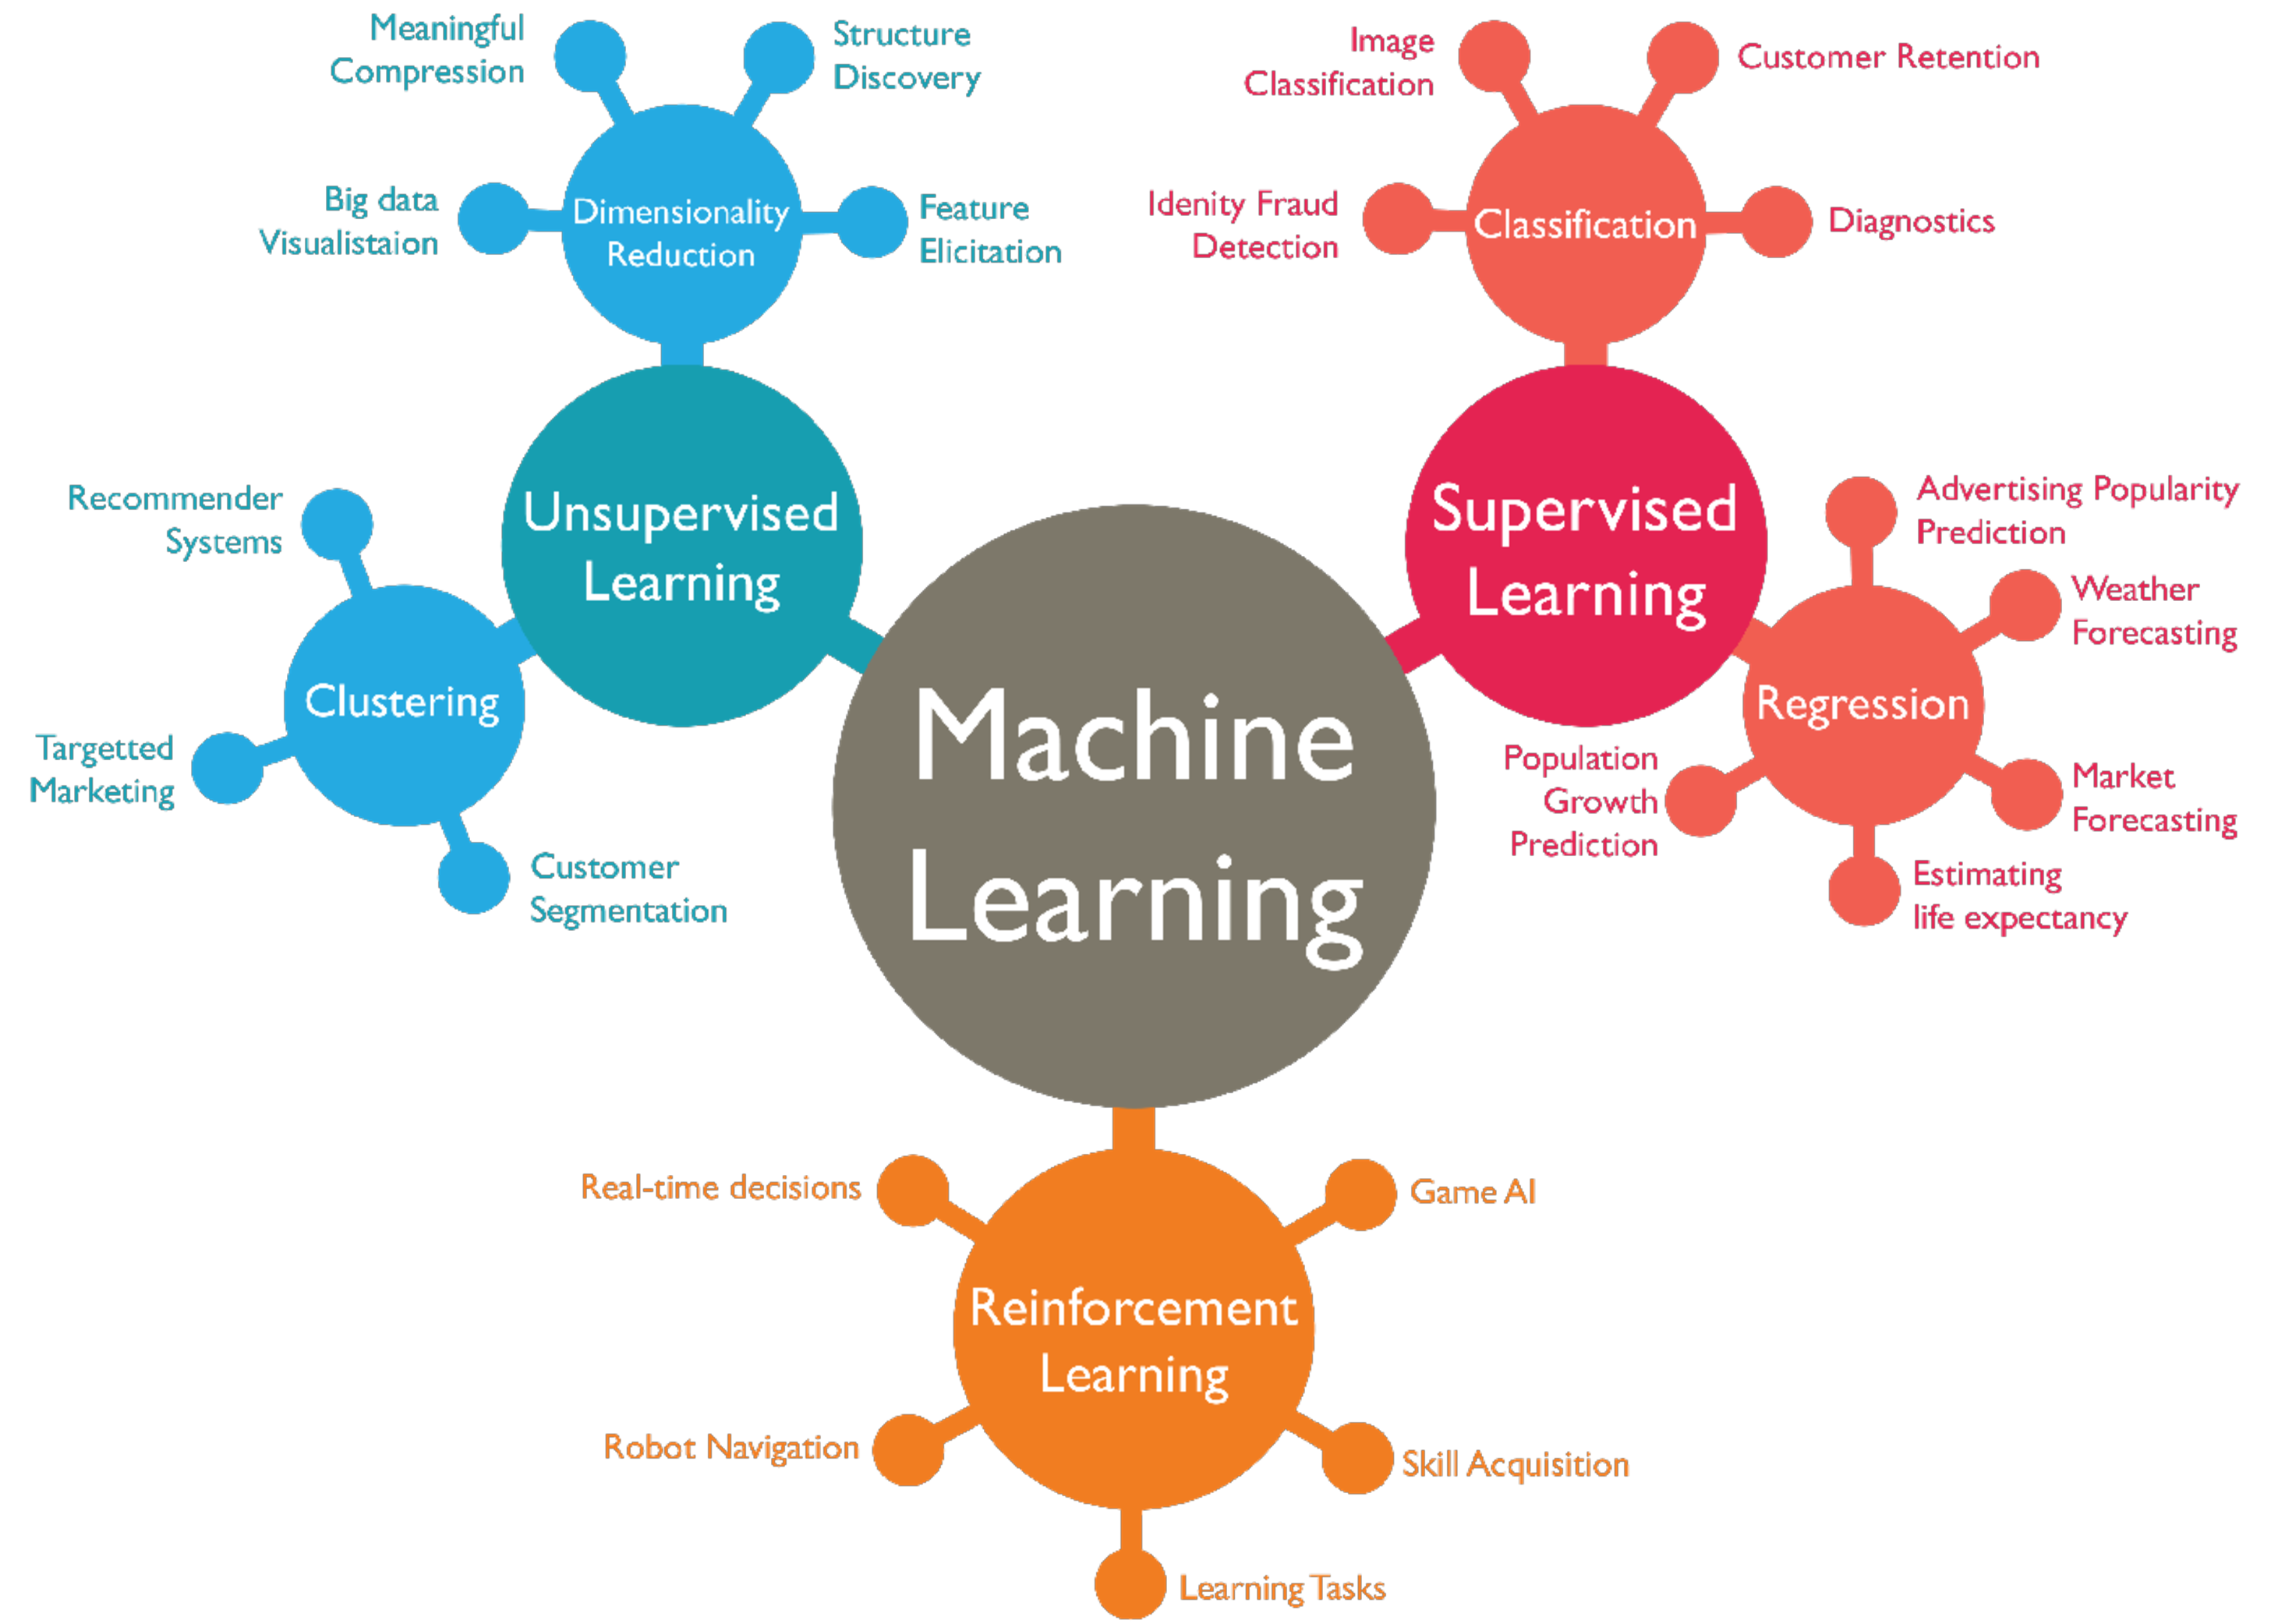
\includegraphics[width=0.7\textwidth]{fig/ml.pdf}
    \end{figure}
\end{frame}
%%% SLIDE %%%

%%% SLIDE %%%
\begin{frame}
	\Huge Como aplicar AM?
\end{frame}
%%% SLIDE %%%

%%% SLIDE %%%
\begin{frame}{Como aplicar AM?}
    \only<1>{
	    \begin{figure}
		    
\includegraphics[width=0.3\paperwidth]{fig/python.jpg}
		    \caption{\href{http://www.python.org}{http://www.python.org}}
	    \end{figure}
	}
	
	\only<2>{
	    \begin{figure}
		    
\includegraphics[width=0.3\paperwidth]{fig/jupyter.jpg}
		    \caption{\href{http://www.jupyter.org}{http://www.jupyter.org}}
	    \end{figure}
	}
	
	\only<3>{
	    \begin{figure}
		    
\includegraphics[width=0.5\paperwidth]{fig/anaconda.jpg}
		    \caption{\href{http://www.anaconda.com}{http://www.anaconda.com}}
	    \end{figure}
	}
	
	\only<4>{
	    \begin{figure}
		    
\includegraphics[width=0.4\paperwidth]{fig/TensorFlow.pdf}
		    \caption{\href{https://www.tensorflow.org}{https://www.tensorflow.org}}
	    \end{figure}
	}
	
	\only<5>{
	    \begin{figure}
		    
\includegraphics[width=0.35\paperwidth]{fig/keras.jpg}
		    \caption{\href{https://keras.io/}{https://keras.io/}}
	    \end{figure}
	}
	
    \only<6>{
	    \begin{figure}
		    
\includegraphics[width=0.5\paperwidth]{fig/scikit_learn.jpg}
		    \caption{\href{https://scikit-learn.org}{https://scikit-learn.org}}
	    \end{figure}
	}
	
	\only<7>{
	    \begin{figure}
		    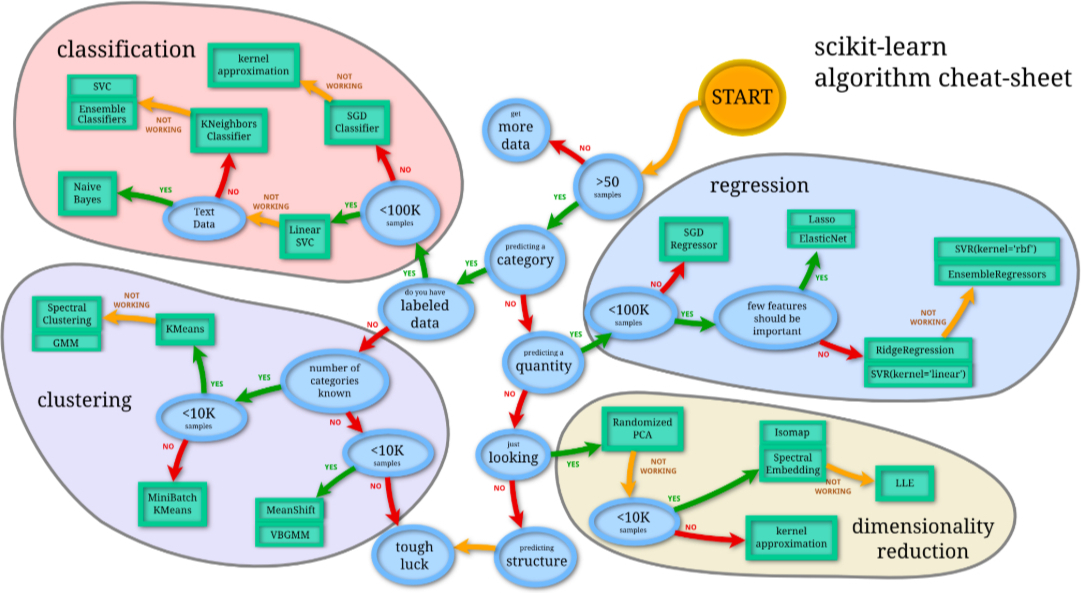
\includegraphics[width=0.7\paperwidth]{fig/scikit_learn_tasks.jpg}
	    \end{figure}
	}
\end{frame}
%%% SLIDE %%%

%%% SLIDE %%%
\begin{frame}{Exemplo}
    \begin{figure}
	    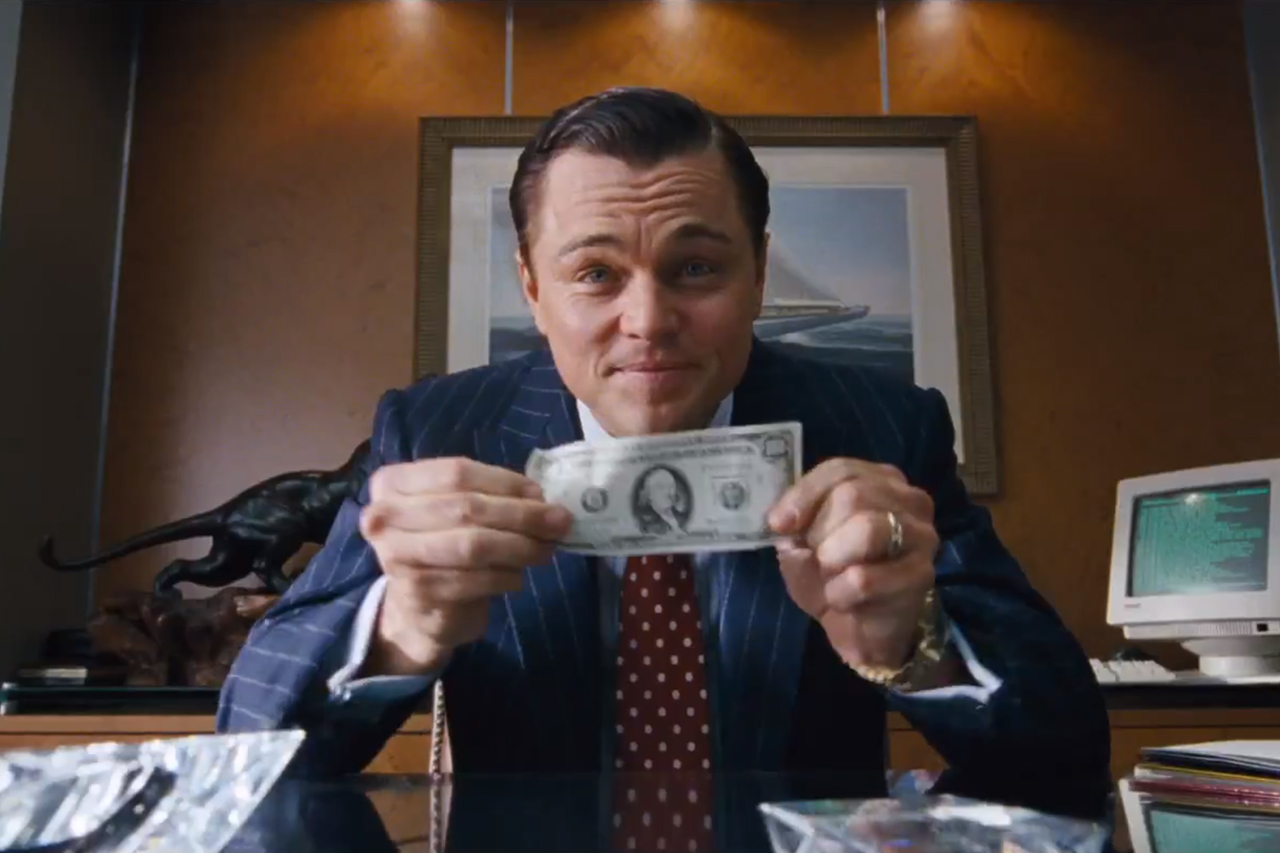
\includegraphics[width=0.55\paperwidth]{fig/dicaprio.jpg}
	    \caption{Dinheiro torna as pessoas felizes?}
    \end{figure}
\end{frame}
%%% SLIDE %%%

%%% SLIDE %%%
\begin{frame}
	\Huge Em suma, em AM...
\end{frame}
%%% SLIDE %%%

%%% SLIDE %%%
\begin{frame}{Em suma, em AM...}
    \begin{itemize}
        \item Estudamos o dado;
        \item Definimos como será o SAM;
        \item Treinamos o SAM (Encontramos os parâmetros que minimizam/maximiza a função custo/utilidade);
        \item Fazemos previsões para novos casos.
    \end{itemize}
\end{frame}
%%% SLIDE %%%

%%% SLIDE %%%
\begin{frame}
    \begin{figure}
        
\includegraphics[width=0.9\textwidth]{fig/hastalavistababy.jpg}
    \end{figure}
\end{frame}
%%% SLIDE %%%

\end{document}
